% *** Authors should verify (and, if needed, correct) their LaTeX system  ***
% *** with the testflow diagnostic prior to trusting their LaTeX platform ***
% *** with production work. IEEE's font choices can trigger bugs that do  ***
% *** not appear when using other class files.                            ***
% The testflow support page is at:
% http://www.michaelshell.org/tex/testflow/


%%*************************************************************************
%% Legal Notice:
%% This code is offered as-is without any warranty either expressed or
%% implied; without even the implied warranty of MERCHANTABILITY or
%% FITNESS FOR A PARTICULAR PURPOSE!
%% User assumes all risk.
%% In no event shall IEEE or any contributor to this code be liable for
%% any damages or losses, including, but not limited to, incidental,
%% consequential, or any other damages, resulting from the use or misuse
%% of any information contained here.
%%
%% All comments are the opinions of their respective authors and are not
%% necessarily endorsed by the IEEE.
%%
%% This work is distributed under the LaTeX Project Public License (LPPL)
%% ( http://www.latex-project.org/ ) version 1.3, and may be freely used,
%% distributed and modified. A copy of the LPPL, version 1.3, is included
%% in the base LaTeX documentation of all distributions of LaTeX released
%% 2003/12/01 or later.
%% Retain all contribution notices and credits.
%% ** Modified files should be clearly indicated as such, including  **
%% ** renaming them and changing author support contact information. **
%%
%% File list of work: IEEEtran.cls, New_IEEEtran_how-to.pdf, bare_jrnl_new_sample4.tex,
%%*************************************************************************
\PassOptionsToPackage{unicode}{hyperref}
\PassOptionsToPackage{hyphens}{url}
\PassOptionsToPackage{dvipsnames,svgnames,x11names}{xcolor}
% Note that the a4paper option is mainly intended so that authors in
% countries using A4 can easily print to A4 and see how their papers will
% look in print - the typesetting of the document will not typically be
% affected with changes in paper size (but the bottom and side margins will).
% Use the testflow package mentioned above to verify correct handling of
% both paper sizes by the user's LaTeX system.
%
% Also note that the "draftcls" or "draftclsnofoot", not "draft", option
% should be used if it is desired that the figures are to be displayed in
% draft mode.
%
\documentclass[
  10pt,
  conference,
]{IEEEtran}%
% If IEEEtran.cls has not been installed into the LaTeX system files,
% manually specify the path to it like:
% \documentclass[journal]{../sty/IEEEtran}
\usepackage{xparse}
\usepackage[cmex10]{amsmath}
\usepackage{amssymb}
\usepackage{iftex}
\ifPDFTeX
  \usepackage[T1]{fontenc}
  \usepackage[utf8]{inputenc}
  \usepackage{textcomp} % provide euro and other symbols
\else % if luatex or xetex
  \usepackage{unicode-math} % this also loads fontspec
  \defaultfontfeatures{Scale=MatchLowercase}
  \defaultfontfeatures[\rmfamily]{Ligatures=TeX,Scale=1}
\fi
%\usepackage{lmodern}
\ifPDFTeX\else
\fi
% Use upquote if available, for straight quotes in verbatim environments
\IfFileExists{upquote.sty}{\usepackage{upquote}}{}
\IfFileExists{microtype.sty}{% use microtype if available
  \usepackage[]{microtype}
  \UseMicrotypeSet[protrusion]{basicmath} % disable protrusion for tt fonts
}{}
\makeatletter
\parindent    1.0em
\ifCLASSOPTIONcompsoc
  \parindent    1.5em
\fi
\makeatother
\usepackage{xcolor}
\setlength{\emergencystretch}{3em} % prevent overfull lines

\setcounter{secnumdepth}{5}
% Make \paragraph and \subparagraph free-standing
\ifx\paragraph\undefined\else
  \let\oldparagraph\paragraph
  \renewcommand{\paragraph}[1]{\oldparagraph{#1}\mbox{}}
\fi
\ifx\subparagraph\undefined\else
  \let\oldsubparagraph\subparagraph
  \renewcommand{\subparagraph}[1]{\oldsubparagraph{#1}\mbox{}}
\fi


\providecommand{\tightlist}{%
  \setlength{\itemsep}{0pt}\setlength{\parskip}{0pt}}\usepackage{longtable,booktabs,array}
\usepackage{calc} % for calculating minipage widths
% Correct order of tables after \paragraph or \subparagraph
\usepackage{etoolbox}
\makeatletter
\patchcmd\longtable{\par}{\if@noskipsec\mbox{}\fi\par}{}{}
\makeatother
% Allow footnotes in longtable head/foot
\IfFileExists{footnotehyper.sty}{\usepackage{footnotehyper}}{\usepackage{footnote}}
\makesavenoteenv{longtable}
\usepackage{graphicx}
\makeatletter
\newsavebox\pandoc@box
\newcommand*\pandocbounded[1]{% scales image to fit in text height/width
  \sbox\pandoc@box{#1}%
  \Gscale@div\@tempa{\textheight}{\dimexpr\ht\pandoc@box+\dp\pandoc@box\relax}%
  \Gscale@div\@tempb{\linewidth}{\wd\pandoc@box}%
  \ifdim\@tempb\p@<\@tempa\p@\let\@tempa\@tempb\fi% select the smaller of both
  \ifdim\@tempa\p@<\p@\scalebox{\@tempa}{\usebox\pandoc@box}%
  \else\usebox{\pandoc@box}%
  \fi%
}
% Set default figure placement to htbp
\def\fps@figure{htbp}
\makeatother
% definitions for citeproc citations
\NewDocumentCommand\citeproctext{}{}
\NewDocumentCommand\citeproc{mm}{%
  \begingroup\def\citeproctext{#2}\cite{#1}\endgroup}
\makeatletter
 % allow citations to break across lines
 \let\@cite@ofmt\@firstofone
 % avoid brackets around text for \cite:
 \def\@biblabel#1{}
 \def\@cite#1#2{{#1\if@tempswa , #2\fi}}
\makeatother
\newlength{\cslhangindent}
\setlength{\cslhangindent}{1.5em}
\newlength{\csllabelwidth}
\setlength{\csllabelwidth}{3em}
\newenvironment{CSLReferences}[2] % #1 hanging-indent, #2 entry-spacing
 {\begin{list}{}{%
  \setlength{\itemindent}{0pt}
  \setlength{\leftmargin}{0pt}
  \setlength{\parsep}{0pt}
  % turn on hanging indent if param 1 is 1
  \ifodd #1
   \setlength{\leftmargin}{\cslhangindent}
   \setlength{\itemindent}{-1\cslhangindent}
  \fi
  % set entry spacing
  \setlength{\itemsep}{#2\baselineskip}}}
 {\end{list}}
\usepackage{calc}
\newcommand{\CSLBlock}[1]{\hfill\break\parbox[t]{\linewidth}{\strut\ignorespaces#1\strut}}
\newcommand{\CSLLeftMargin}[1]{\parbox[t]{\csllabelwidth}{\strut#1\strut}}
\newcommand{\CSLRightInline}[1]{\parbox[t]{\linewidth - \csllabelwidth}{\strut#1\strut}}
\newcommand{\CSLIndent}[1]{\hspace{\cslhangindent}#1}

\usepackage{booktabs}
\usepackage{longtable}
\usepackage{array}
\usepackage{multirow}
\usepackage{wrapfig}
\usepackage{float}
\usepackage{colortbl}
\usepackage{pdflscape}
\usepackage{tabu}
\usepackage{threeparttable}
\usepackage{threeparttablex}
\usepackage[normalem]{ulem}
\usepackage{makecell}
\usepackage{xcolor}
\usepackage{physics}
\usepackage[version=3]{mhchem}
\usepackage{orcidlink}
\usepackage{float}
\floatplacement{table}{htb}
\makeatletter
\@ifpackageloaded{tcolorbox}{}{\usepackage[skins,breakable]{tcolorbox}}
\@ifpackageloaded{fontawesome5}{}{\usepackage{fontawesome5}}
\definecolor{quarto-callout-color}{HTML}{909090}
\definecolor{quarto-callout-note-color}{HTML}{0758E5}
\definecolor{quarto-callout-important-color}{HTML}{CC1914}
\definecolor{quarto-callout-warning-color}{HTML}{EB9113}
\definecolor{quarto-callout-tip-color}{HTML}{00A047}
\definecolor{quarto-callout-caution-color}{HTML}{FC5300}
\definecolor{quarto-callout-color-frame}{HTML}{acacac}
\definecolor{quarto-callout-note-color-frame}{HTML}{4582ec}
\definecolor{quarto-callout-important-color-frame}{HTML}{d9534f}
\definecolor{quarto-callout-warning-color-frame}{HTML}{f0ad4e}
\definecolor{quarto-callout-tip-color-frame}{HTML}{02b875}
\definecolor{quarto-callout-caution-color-frame}{HTML}{fd7e14}
\makeatother
\makeatletter
\@ifpackageloaded{caption}{}{\usepackage{caption}}
\AtBeginDocument{%
\ifdefined\contentsname
  \renewcommand*\contentsname{Table of contents}
\else
  \newcommand\contentsname{Table of contents}
\fi
\ifdefined\listfigurename
  \renewcommand*\listfigurename{List of Figures}
\else
  \newcommand\listfigurename{List of Figures}
\fi
\ifdefined\listtablename
  \renewcommand*\listtablename{List of Tables}
\else
  \newcommand\listtablename{List of Tables}
\fi
\ifdefined\figurename
  \renewcommand*\figurename{Fig.}
\else
  \newcommand\figurename{Fig.}
\fi
\ifdefined\tablename
  \renewcommand*\tablename{Table}
\else
  \newcommand\tablename{Table}
\fi
}
\@ifpackageloaded{float}{}{\usepackage{float}}
\floatstyle{ruled}
\@ifundefined{c@chapter}{\newfloat{codelisting}{h}{lop}}{\newfloat{codelisting}{h}{lop}[chapter]}
\floatname{codelisting}{Listing}
\newcommand*\listoflistings{\listof{codelisting}{List of Listings}}
\makeatother
\makeatletter
\makeatother
\makeatletter
\@ifpackageloaded{caption}{}{\usepackage{caption}}
\@ifpackageloaded{subcaption}{}{\usepackage{subcaption}}
\makeatother

\usepackage[skip=2pt,font=footnotesize]{caption}
%\captionsetup{format=myformat}
\makeatletter
%\setlength{\cslhangindent}{0pt plus .5pt}
\providecommand{\bibfont}{\footnotesize}
\let\CSLReferences@rig=\CSLReferences
\renewcommand{\CSLReferences}[2]{
\bibfont\settowidth\csllabelwidth{[999]}
\CSLReferences@rig{#1}{#2}
\vskip 0.3\baselineskip plus 0.1\baselineskip minus 0.1\baselineskip%
}
\makeatother
\ifLuaTeX
  \usepackage{selnolig}  % disable illegal ligatures
\fi
\IfFileExists{bookmark.sty}{\usepackage{bookmark}}{\usepackage{hyperref}}
\IfFileExists{xurl.sty}{\usepackage{xurl}}{} % add URL line breaks if available
\urlstyle{same} % disable monospaced font for URLs
\hypersetup{
  pdftitle={Exploring How SE Academic Papers Use Figures},
  pdfauthor={Marco Torchiano; Lorenzo Laudadio},
  pdfkeywords={visualization, software engineering},
  colorlinks=true,
  linkcolor={blue},
  filecolor={Maroon},
  citecolor={Blue},
  urlcolor={Blue},
  pdfcreator={LaTeX via pandoc}}

% *** Do not adjust lengths that control margins, column widths, etc. ***
% *** Do not use packages that alter fonts (such as pslatex).         ***
% There should be no need to do such things with IEEEtran.cls V1.6 and later.
% (Unless specifically asked to do so by the journal or conference you plan
% to submit to, of course. )


% correct bad hyphenation here
\hyphenation{op-tical net-works semi-conduc-tor}

%
% paper title
% can use linebreaks \\ within to get better formatting as desired
% Do not put math or special symbols in the title.
% paper title
% can use linebreaks \\ within to get better formatting as desired
% Do not put math or special symbols in the title.
\title{Exploring How SE Academic Papers Use Figures}

\author{
\IEEEauthorblockN{Marco Torchiano}
\IEEEauthorblockA{%
            Computer and Control Engineering\\
            \textit{Politecnico di Torino}\\
            Torino  10129\\
             Italy      \\
marco.torchiano@polito.it
\orcidlink{0000-0001-5328-368X}
}\and
\IEEEauthorblockN{Lorenzo Laudadio}
\IEEEauthorblockA{%
            Computer and Control Engineering\\
            \textit{Politecnico di Torino}\\
            Torino  10129\\
             Italy      \\
lorenzo.laudadio@polito.it
\orcidlink{0009-0001-3496-0072}
}
}
\begin{document}

% The paper headers
\markboth{WSESE 2025}{Torchiano et al.: Exploring How SE Academic Papers
Use Figures}

% use for special paper notices

% make the title area
\maketitle

% As a general rule, do not put math, special symbols or citations
% in the abstract or keywords.
\begin{abstract}
The usage of figures to represent data or concepts in scientific
articles is a common practice. We aim to understand what figures are
used for in SE articles and in particular how quantitative data is
represented. For this purpose we analyzed 865 articles published in
leading software engineering scientific conferences and journals and
classified 6342 figures and their contents. 47\% of the figures are used
to convey quantitative information and the rest depict more abstract
non-quantitative information. The most common types of quantitative
diagrams are bar plots, box plots, and line plots, accounting for 75\%
of the quantitative figures. We also found that each figure contains 1.6
errors, although 75\% of them do not contain any critical error.
Critical blatant errors are found in less than 5\% of the figures.
\end{abstract}
% Note that keywords are not normally used for peerreview papers.
\begin{IEEEkeywords}
visualization, software engineering
\end{IEEEkeywords}

% For peer review papers, you can put extra information on the cover
% page as needed:
% \ifCLASSOPTIONpeerreview
% \begin{center} \bfseries EDICS Category: 3-BBND \end{center}
% \fi
%
% For peerreview papers, this IEEEtran command inserts a page break and
% creates the second title. It will be ignored for other modes.
% \IEEEpeerreviewmaketitle


\section{Introduction}\label{introduction}

In software engineering (SE) research, the effective communication of
ideas, methodologies, and results is paramount. Papers in this field
often employ a variety of visual aids, including figures, tables, and
code fragments, to complement the textual content and enhance clarity.
While there exist a large research community that explores innovative
visualization techniques, the majority of visualizations in SE papers
remain relatively mundane, relying on basic, well-established methods.
This reliance on standard visual aids reflects both the practical
constraints and the entrenched practices within the field.

Practitioners who regularly writes papers and supervises younger
researchers, can often find themselves providing guidance on the
effective use of visualizations. This necessity arises from observing a
recurring issue: poorly designed diagrams that fail to effectively
convey the intended information. Additionally, as reviewers, we
frequently encounter diagrams that are not only visually unappealing but
also ineffective in communicating complex ideas. These experiences
underscore a broader concern within the community regarding the
presentation quality of SE papers. A critical question emerges: is it
worthwhile to invest substantial effort in designing more sophisticated
and effective diagrams? This paper aims to address this question by
examining the current state of visualization practices in SE research.

The goal of this paper is to advance the discourse on visualization in
software engineering. The main contributions consist in:

\begin{itemize}
\tightlist
\item
  Overview of the State of the Practice: We provide a comprehensive
  analysis of the current visualization practices within prominent SE
  venues, identifying prevailing trends and common practices.
\item
  Purpose of Figures: An examination of the various roles that figures
  play in SE papers, shedding light on how they contribute to the
  overall narrative and understanding of the research.
\item
  Catalogue of Common Diagrams: A detailed catalog of the most
  frequently used diagrams, offering insights into their typical
  applications and variations.
\end{itemize}

In particular we will focus on quantitative visualization, i.e.~charts
and diagrams that encode quantitative measures. This is opposed to
non-quantitative visualization that represent conceptual aspects in a
more or less formal way, e.g., software representations such as UML
diagrams.

Overall by surveying the current practices and identifying most common
errors, this paper seeks to elevate the standard of visual communication
in software engineering research, ultimately contributing to the clarity
and impact of published work.

\section{Background}\label{background}

Data visualization is a critical component in the communication of
scientific research, enabling the distillation of complex data into
comprehensible visual formats. By transforming raw data into graphical
representations, researchers can more effectively highlight patterns,
trends, and anomalies, thereby facilitating better understanding and
interpretation. In the context of academic publications, well-designed
visualizations are not merely supplementary but essential elements that
enhance the clarity and impact of the presented research.

\subsection{Visualization of Quantitative
Information}\label{visualization-of-quantitative-information}

The seminal book \emph{The Visual Display of Quantitative Information}
\citeproc{ref-tufte1983}{{[}1{]}} revolutionized the way quantitative
data is presented. Tufte emphasized principles such as lie factor and
data-ink ratio, and laid the groundwork for a set of best practices that
prioritize proportionality, clarity, and utility in the visual
representation of data.

Building on the principles established by Tufte, subsequent scholars
have further refined the guidelines for effective data visualization.
Notably, Tamara Munzner's \emph{Visualization Analysis and Design}
\citeproc{ref-munzner2014}{{[}2{]}} offers a comprehensive framework for
creating insightful and effective visualizations. Munzner's work
addresses the complexity of visual encoding and interaction, providing a
systematic approach to design that is applicable across various
disciplines. Her guidelines cover a broad spectrum of visualization
types, from simple charts to complex, interactive graphics, emphasizing
the importance of aligning visualization techniques with the specific
needs and goals of the analysis.

In the domain of software engineering (SE), tailored guidelines for
visualization have been proposed to address the unique challenges and
requirements of the field. One notable contribution is the Empirical
Standards for Software Engineering Research, as articulated by
\citeproc{ref-EmpiricalStandards}{{[}3{]}}. These standards provide a
robust framework for conducting and presenting empirical research in SE,
including specific recommendations for the use of visualizations. The
guidelines emphasize aim to ensure that dagrams and charts effectively
support the communication of research findings.

\subsection{Graph Error Taxonomy}\label{sec-error-taxonomy}

On the basis of the extensive literature and the personal experience in
reviewing papers we defined a taxonomy of errors that include three
levels of severity:

\begin{itemize}
\tightlist
\item
  Critical: the error can severely impact the correct understanding of
  the quantitative message;
\item
  Major: the error can significantly impact the ease of understanding,
  demanding more effort than strictly required;
\item
  Minor: the error can moderately impact the ease of understanding.
\end{itemize}

A summary of the errors we identified, divided by severity is reported
in table Table~\ref{tbl-errors}.

\begin{table}

\caption{\label{tbl-errors}Summary of errors by severity level.}

\centering{

\begin{tabular}[t]{lp{0.8\linewidth}lp{0.8\linewidth}}
\toprule
Severity & Errors\\
\midrule
Critical & Cropped, Deformed, DoubleScale,
MissingAxesRef, NonZeroBased,
SimilarColors, TooManyCats\\
Major & 3D, GridDistinctRanges,
InterruptedScale, Legend, Mislabeled,
Overplotting, RotatedXLabels, SilentLog,
Unlabeled\\
Minor & ColorsUncoded, HeavyBackground,
HeavyGrid, LegendBorder, LegendInside,
OverlappedLabels, PatternFill, Raster,
Shadow, TooMuchPrecision, WasteSpace,
WrappedXLabs\\
\bottomrule
\end{tabular}

}

\end{table}%

The detailed descriptions of the are reported below:

\subsubsection{Critical}\label{critical}

\begin{itemize}
\item
  \textbf{Cropped} The graph is cropped and some details are not visible
  since they lay outside. This impedes the vision of part of the
  diagram.
\item
  \textbf{Deformed} The graph is somehow deformed with proportion not
  consistente across the area. Often this is -- wrongly -- used to
  emphasize some detail instead of using more suitable techniques, the
  reuslt is a deception of the observer
  \citeproc{ref-pandey2015}{{[}4{]}}.
\item
  \textbf{DoubleScale} The graph uses a double (vertical) scale.
  Research in cognitive science \citeproc{ref-Few2012}{{[}5{]}} suggests
  that people may misinterpret trends if they do not notice the
  differing scales, potentially leading to incorrect conclusions about
  the correlation between the two datasets.
\item
  \textbf{MissingAxesRef} The whole axes or the tick marks are missing.
  This make the quantitative information contained in the diagram fuzzy
  and imprecise failing the goal of conveying accurate information.
\item
  \textbf{NonZeroBased} A bar diagram with truncated bars, axis not
  starting at 0. This is a serious problem concerning the visual
  integrity of the diagram, in particualar it affects proportionality
  \citeproc{ref-tufte1983}{{[}1{]}}, thus falsifying the quantitative
  message of the diagram.
\item
  \textbf{SimilarColors} Graph uses very similar colors, hard to tell
  apart. Research indicates that low contrast between colors (especially
  in terms of luminosity) can reduce the speed and accuracy of
  information interpretation \citeproc{ref-silva2011}{{[}7{]}}.
\item
  \textbf{TooManyCats} The graph encodes too many categories (usually
  more than six) with attributes like color or shape. For instance,
  \citeproc{ref-macdonald1999}{{[}8{]}} recommends that the number of
  colors used to represent nominal data should be restricted to seven or
  less, while sudies by \citeproc{ref-ware2013}{{[}6{]}} found that
  people can typically distinguish 4 to 6 distinct shapes effectively.
\end{itemize}

\subsubsection{Major}\label{major}

\begin{itemize}
\item
  \textbf{3D} There are 3D effects. The additional cognitive effort
  required for 3D interpretation often results in slower reaction times
  and higher error rates \citeproc{ref-ware2013}{{[}6{]}}.
\item
  \textbf{GridDistinctRanges} When multiple graph are present (grid of
  chars, a.k.a. small multiples), the corresponding axes have different
  intervals. \citeproc{ref-heer2009}{{[}9{]}} shows that when the scales
  are consistent across all plots, viewers can quickly and accurately
  compare values; while inconsistent axes may lead to misinterpretation.
\item
  \textbf{InterruptedScale} One of the axes is interrupted and restarted
  after a discontinuity to show extremely spread values. Axis breaks can
  affect the perceived effect size, leading viewers to believe that the
  differences between data points are more significant than they
  actually are \citeproc{ref-pandey2015}{{[}4{]}}.
\item
  \textbf{Legend} There is a legend that could have been turned into
  direct labeling. Direct labeling (i.e., placing labels close to the
  data points) instead of using a separate legend reduces the need for
  eye movements between the legend and the chart elements, thus it leads
  to faster and more accurate interpretation
  \citeproc{ref-ratwani2008}{{[}10{]}}.
\item
  \textbf{Mislabeled} Labels are obscuring or get confused with data. A
  key recommendation when creating a diagram is `above all show the
  data' \citeproc{ref-tufte1983}{{[}1{]}}.
\item
  \textbf{Overplotting} There are too many overplotted points that
  prevent distinguishing individual points. It leads to misleading
  interpretations, particularly in scatter plots used to show
  relationships or correlations; since the points are not
  distinguishable, viewers may fail to detect underlying relationships
  or trends \citeproc{ref-Few2012}{{[}5{]}}.
\item
  \textbf{RotatedXLabels} The labels on the X axis are rotated (not
  horizontal). Rotated labels can interfere with the viewer's ability to
  quickly interpret the data, as they require additional time for visual
  decoding; such effect is particularly pronounced in bar charts with
  long category labels \citeproc{ref-Few2012}{{[}5{]}}.
\item
  \textbf{SilentLog} One of the axes uses a log scale but this is not
  clearly mentioned. While log scales help in visualizing both small and
  large values in the same plot without extreme compression or skewing
  of the data points \citeproc{ref-cleveland1994}{{[}11{]}}, viewers
  often misinterpret log scales if the axis labels do not clearly
  indicate the logarithmic nature of the scale
  \citeproc{ref-Few2012}{{[}5{]}}.
\item
  \textbf{Unlabeled} The axes are not labeled. While the meaning of the
  axes can be inferred from the caption of the main text of the article,
  the lack of labels makes understanding the graph much less immediate.
\end{itemize}

\subsubsection{Minor}\label{minor}

\begin{itemize}
\item
  \textbf{ColorsUncoded} There are many color not corresponding to an
  explicit coding (legend or other). If colors are used purely for
  decorative purposes without encoding information, they may
  inadvertently create a false visual hierarchy, drawing attention away
  from the key data elements \citeproc{ref-Few2012}{{[}5{]}}.
\item
  \textbf{HeavyBackground} The background is heavy. If the background is
  so intense to almost obscure the data or to draw attention away from
  the data, the visual message is lost
  \citeproc{ref-tufte1983}{{[}1{]}}.
\item
  \textbf{HeavyGrid} The grid of the graph is heavy. If the visual
  presence of grid is so strong to almost obscure the data, the visual
  message is lost \citeproc{ref-tufte1983}{{[}1{]}}.
\item
  \textbf{LegendBorder} The legend has a border (preventing free eye
  scan)
\item
  \textbf{LegendInside} The legeng is inside the graph area
\item
  \textbf{OverlappedLabels} Labels are overlapping with each other.
  Overlapping labels are difficult to read thus they require additional
  effort or make impossible understanding.
\item
  \textbf{PatternFill} Area fill is using a parttern (e.g., lines or
  dots) instead of diferent hues or gray levels. Excessive use of
  patterns can create a `busy' appearance, making it harder for viewers
  to focus on the main data trends \citeproc{ref-Few2012}{{[}5{]}}.
\item
  \textbf{Raster} Usage of low resolution raster images instead of
  vectorial format. When a figure uses a raster image with poor
  resolution it appears unpleasantly grainy -- espectially when zoomed
  in -- and possibly difficult to read.
\item
  \textbf{Shadow} The graph makes use of shadows. Using shadows as well
  as other decorative visual effects reduces the data-to-ink ratio and
  makes the diagram cluttered, thus weakening the visual message
  \citeproc{ref-tufte1983}{{[}1{]}}.
\item
  \textbf{TooMuchPrecision} The graph reports values that have a too
  high precision (decimal digits) for the intended purpose. Any
  additional information that is not necessary increases the cognitive
  load and makes the graph less understandable
  \citeproc{ref-Few2012}{{[}5{]}}.
\item
  \textbf{WasteSpace} A large portion of graph area is empty. This is a
  bad us of space that dilutes the visual message in the graph.
\item
  \textbf{WrappedXLabs} Labels on the x axis are wrapped due to limited
  space. Wrapped labels are more difficult to read, often they can be
  solved with a simple graph redesign.
\end{itemize}

\section{Experimental design}\label{experimental-design}

The general goal of the study can be formulated using the GQM template
\citeproc{ref-GQM1999}{{[}12{]}}:

\begin{table}

\caption{\label{tbl-GQM}GQM definition}

\centering{

\begin{tabular}[t]{ll}
\toprule
 & \\
\midrule
Analyze & the usage of figures articles\\
For the purpose of & understanding\\
With respect to & the type, technique, and mistakes\\
From the viewpoint of & paper authors and reviewers\\
In the context of & SE conferences and journals\\
\bottomrule
\end{tabular}

}

\end{table}%

\subsection{Research questions}\label{research-questions}

In order to achieve the above goal we define the following research
questions:

\begin{itemize}
\item
  \textbf{RQ1}. Mode: how are figures used in SE articles?

  To have an initial assessment of the phenomenon we consider important
  to understand how many figures are used in SE papers. Also it is
  interesting to observe if there is a trend in time concerning the
  usage of figures.
\item
  \textbf{RQ2}. Content: what are figures used for?

  Figures are used to convey many different types of information. The
  most general distinction is between quantitative and non quantitative
  information. A further step is to look into the different type of
  contents shown in the figures.
\item
  \textbf{RQ3}. Type: what types of diagrams are used to convey
  quantitative information?

  Focusing on quantitative diagrams we investigate the type of diagrams
  used in the papers.
\item
  \textbf{RQ4}. Mistakes: What are the errors committed in quantitative
  diagrams?

  We focus on all diagrams and then we analyze the specific mistakes
  committed in the most used diagram types.
\end{itemize}

For all the question above we aim to investigate whether a change can be
observed for different venues and if time affected any aspect.

\subsection{Variables}\label{sec-variables}

To investigate the above research questions we collected a set of
variables that are described in Table~\ref{tbl-variables}.

In particular we collected measures on two type of entities: the
articles and figures that appear in them.

\begin{table}

\caption{\label{tbl-variables}Variables}

\centering{

\begin{tabular}[t]{lll}
\toprule
Entity & Variable & Description\\
\midrule
Article & VenueType & categorical: \{ Conference, Journal \}\\
 & Venue & string: name of conf. or journal\\
 & Year & integer: year of publication\\
 & Pages & integer: pages of the article\\
 & NumFigures & integer: number of figures\\
 & FigDensity & derived: NumFigures/Pages\\
\midrule
Figure & Category & categorical: \{Q, NonQ\}\\
 & Type & categorical: type of content\\
 & Mistake & set of categorical: the errors found\\
\bottomrule
\end{tabular}

}

\end{table}%

Concerning the figures, in addition to the main distinction between
quantitative (Q) and non-quantitative (NonQ), we categorized the type of
content. The list of types of figure contents are reported in
Table~\ref{tbl-types} divided into quantitative and non quantitative.

\begin{table}

\caption{\label{tbl-types}Types of figures}

\centering{

\begin{tabular}[t]{lp{0.8\linewidth}lp{0.8\linewidth}}
\toprule
Category & Types\\
\midrule
NonQ & Code, Graph, Picture, Schema,
Screenshot, Table, Wordcloud\\
Q & Alluvial, Area, Bar, Bar Grouped,
Bar Stacked, Bar Stacked Diverging,
Beeswarm, Boxplot, Bubble, Bump,
Dendrogram, Donut, Dot, Forest, Heatmap,
Line, Pie, Radar, Scatter, Slope,
Sunburst, Surface, Treemap, Venn, Violin\\
\bottomrule
\end{tabular}

}

\end{table}%

The taxonomy of graph type was initially formed on the basis of the main
graph types described in the literature, e.g.
\citeproc{ref-Few2012}{{[}5{]}}. Then it was updated when, during the
analysis of the articles, a diagram that was impossible to classify
appeared.

\subsection{Procedure}\label{procedure}

We selected a set of recent issues of two leading SE Journals -- IEEE
Transactions on Software Engineering (TSE) and Empirical Software
Engineering Journal (EMSE) -- and SE conferences -- ACM/IEEE
International Symposium on Empirical Software Engineering and
Measurement (ESEM) and ACM/IEEE International Conference on Software
Engineering (ICSE) --. We downloaded all the articles in 2022 issues of
the two journals, those appearing in the year 2017, 2019, 2021, and 2022
of ESEM and a sample of those appearing in years 2018, 2019, 2021, and
2022 of ICSE\footnote{Due to the large number of articles in ICSE, only
  a sample of the total article was analyzed except for year 2019.}. For
each article we went though it and for each figure we classified it
using the taxonomy presented in the section above. In addition, for the
quantitative figures, we applied the error taxonomy described in
Section~\ref{sec-error-taxonomy} to identify errors present in the
figure.

The person performing the analysis started with a limited number of
articles then they discussed all the collected data with the leading
researcher to define the correct application of the taxonomy. After the
processing of a whole venue a second round of discussion focused on the
dubious cases that emerged during the analysis.

\section{Results}\label{results}

Overall in our study we analyzed a total of 865 articles that included
6342 figures. The detailed counts for the different venues we took into
consideration are reported in Table~\ref{tbl-sources}.

\begin{table}

\caption{\label{tbl-sources}Summary of articles and figures analyzed}

\centering{

\begin{tabular}[t]{lllrrr}
\toprule
VenueType & Venue & Year & Figures & Articles & TotalArticles\\
\midrule
Conference & ESEM & 2017 & 180 & 63 & 63\\
 &  & 2019 & 183 & 48 & 48\\
 &  & 2021 & 143 & 24 & 24\\
 &  & 2022 & 123 & 24 & 24\\
\addlinespace
 & ICSE & 2018 & 95 & 14 & 152\\
 &  & 2019 & 641 & 109 & 109\\
 &  & 2021 & 209 & 38 & 138\\
 &  & 2022 & 584 & 69 & 99\\
\addlinespace
Journal & EMSE & 2022 & 1918 & 192 & 192\\
 & TSE & 2022 & 2266 & 284 & 284\\
\addlinespace
 & Total &  & 6342 & 865 & 1133\\
\bottomrule
\end{tabular}

}

\end{table}%

\subsection{RQ1: Mode}\label{rq1-mode}

The first RQ focuses on how much figures are used in SE papers to convey
information.

To address this question we looked at the number of figures that are
used in the articles. Since the length of the articles can be quite
diverse, we computed a derived measure that is the density of figures,
i.e.~the number of figures per page. Fig.~\ref{fig-density} reports the
figure density for the four different venues, i.e.~the conferences ESEM
and ICSE as well as the journals TSE and ICSE. The figure shows the
distribution of density using a boxplot and reports the mean value as a
cross.

\phantomsection\label{cell-fig-density}
\begin{figure}[tb]

\centering{

\pandocbounded{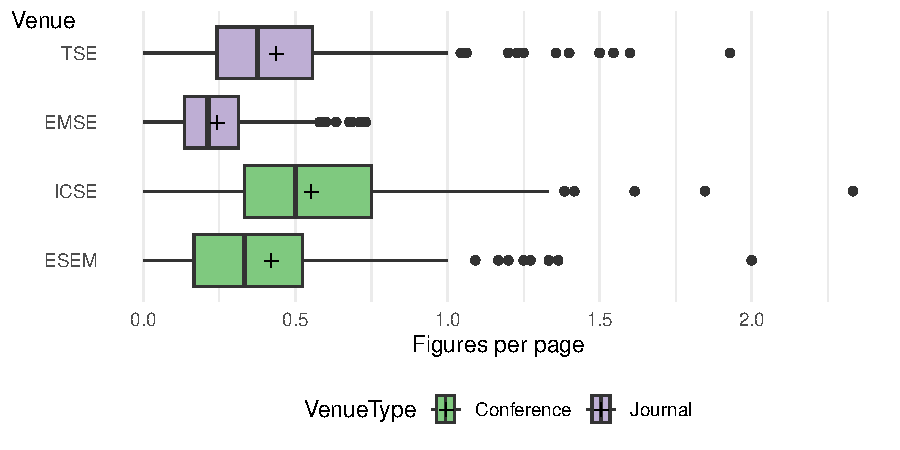
\includegraphics[keepaspectratio]{FiguresSE_files/figure-pdf/fig-density-1.pdf}}

}

\caption{\label{fig-density}Figure density (figures per page) of papers
in different venues}

\end{figure}%

We observe that on average the papers have a mean density of 0.42
figures per page and the median is 0.35. The details are reported in
Table~\ref{tbl-figure-density}. The proportion of articles that have no
picture is 2.9\%, with the highest percentage for ESEM conference
(9.4\%).

\begin{table}

\caption{\label{tbl-figure-density}Summary of figure density by venue}

\centering{

\begin{tabular}[t]{lrrrrl}
\toprule
Venue & Figures & Pages & Mean F/P & Median F/P & w/o Fig\\
\midrule
ESEM & 3.9 & 9.0 & 0.42 & 0.33 & 15 (9.4\%)\\
ICSE & 6.6 & 12.0 & 0.55 & 0.50 & 5 (2.2\%)\\
EMSE & 10.0 & 41.0 & 0.24 & 0.21 & 3 (1.6\%)\\
TSE & 8.0 & 18.3 & 0.44 & 0.38 & 2 (0.7\%)\\
Total & 7.3 & 20.0 & 0.42 & 0.35 & 25 (2.9\%)\\
\bottomrule
\end{tabular}

}

\end{table}%

By looking at the figure we can observe significant differences among
the four venues. Such visual assessment is confirmed by the result of an
ANOVA analysis of figure density vs.~Venue that are reported in
Table~\ref{tbl-anova-density}. Considering as the reference level for
the Venue variable the ESEM conference, by looking at the coefficient
estimates we observe a significantly lower higher value for the ICSE
conference and lower for EMSE journal, while the density of TSE is not
different.

\begin{table}

\caption{\label{tbl-anova-density}ANOVA results of Figure density
vs.~Venue}

\centering{

\begin{tabular}[t]{lrrrl}
\toprule
Coefficient & Estimate & Std. Error & t value & p.value\\
\midrule
(Intercept) & 0.421 & 0.023 & 17.967 & <0.001 ***\\
VenueICSE & 0.131 & 0.030 & 4.309 & <0.001 ***\\
VenueEMSE & -0.177 & 0.032 & -5.596 & <0.001 ***\\
VenueTSE & 0.016 & 0.029 & 0.534 & 0.593\\
\bottomrule
\end{tabular}

}

\end{table}%

Since the length of articles we report in Fig.~\ref{fig-pages-density} a
scatter plot of figure density vs.~number of pages.

\phantomsection\label{cell-fig-pages-density}
\begin{figure}[tb]

\centering{

\pandocbounded{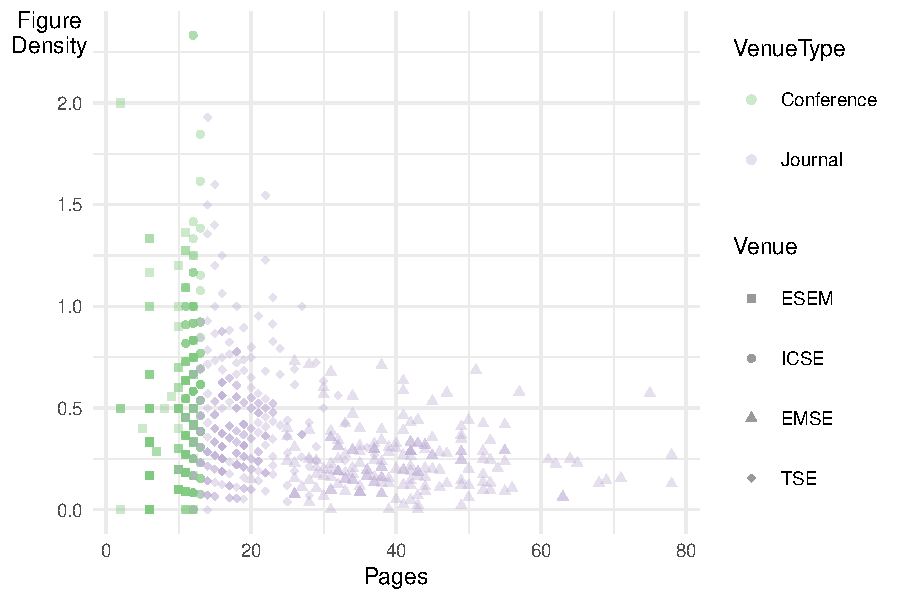
\includegraphics[keepaspectratio]{FiguresSE_files/figure-pdf/fig-pages-density-1.pdf}}

}

\caption{\label{fig-pages-density}Figure density vs.~pages in article
for different venues.}

\end{figure}%

We observe a small negative correlation (Pearson r=-0.273) between the
number of pages and the figure density.

To understand if a change in time occurred we compared the two
conferences over the same years. Fig.~\ref{fig-density-time} reports the
boxplot of density over three years.

\phantomsection\label{cell-fig-density-time}
\begin{figure}[tb]

\centering{

\pandocbounded{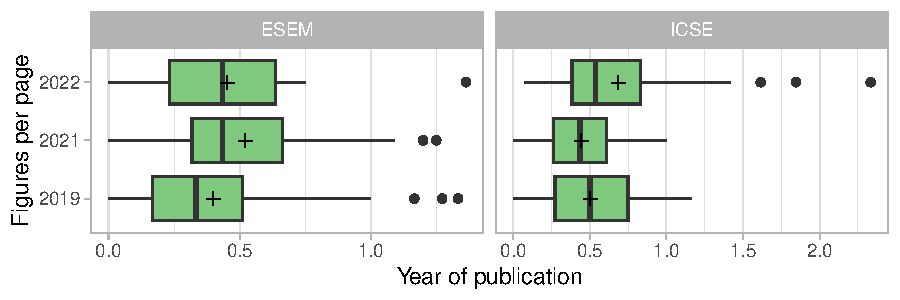
\includegraphics[keepaspectratio]{FiguresSE_files/figure-pdf/fig-density-time-1.pdf}}

}

\caption{\label{fig-density-time}Variation of figure density in
different years}

\end{figure}%

From the figure we can observe a negligible (r=0.138) correlation of
density with year of publication.

\subsection{RQ2 Content}\label{rq2-content}

Fig.~\ref{fig-category-venue} reports the proportion of quantitative (Q)
vs.~non quantitative (NonQ) figures in the article, divided by venue.

\phantomsection\label{cell-fig-category-venue}
\begin{figure}[H]

\centering{

\pandocbounded{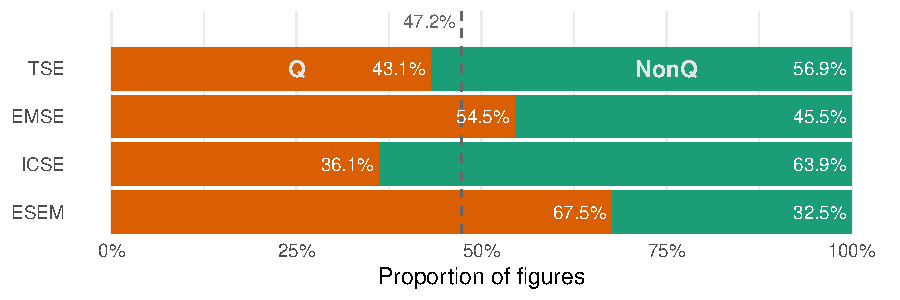
\includegraphics[keepaspectratio]{FiguresSE_files/figure-pdf/fig-category-venue-1.pdf}}

}

\caption{\label{fig-category-venue}Category of figures}

\end{figure}%

Roughly half (47.2\%) of the figures are used to convey quantitative
information while the remaining are used to represent other types of
information. The proportion varies notably among the four venues
considered, with ESEM conference articles having an average of two
thirds figures being quantitative, while ICSE articles invert the
proportion with around one third of quantitative figures.

\phantomsection\label{cell-fig-q-prop}
\begin{figure}[tb]

\centering{

\pandocbounded{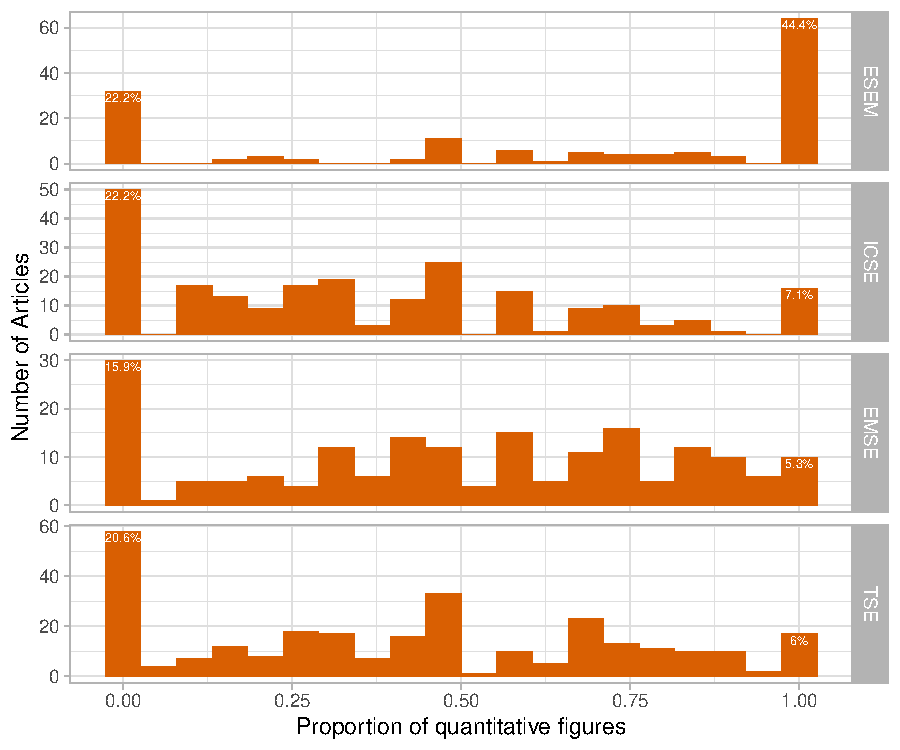
\includegraphics[keepaspectratio]{FiguresSE_files/figure-pdf/fig-q-prop-1.pdf}}

}

\caption{\label{fig-q-prop}Distribution of quantitative figure
proportions}

\end{figure}%

The detailed distribution of the proportion of quantitative figures per
paper is reported in Fig.~\ref{fig-q-prop}. We observe that in the case
of ESEM the distribution is very extreme with 22\% of articles that have
no quantitative figure at all and 44\% that contain only quantitative
figures. For the other venues the proportion articles with only
quantitative figures is much smaller with proportions ranging from 5\%
to 7\%, while the proportion of articles with only non quantitative
figures is close to 20\%.

Focusing on the non quantitative figures only, Fig.~\ref{fig-nonq}
reports the numbers as well as the proportion of the five different non
quantitative types defined in our taxonomy. Two out of three non
quantitative figures fall into the broad \emph{Schema} category that
includes all the diagrams use to explain something, including also
software architecture or UML diagrams. Around one in five \emph{NonQ}
figures are used to depict code, this is common practice used instead of
the \emph{Listing} environment. A smaller proportion (8.2\%) is
represented by screenshots. Eventually, we observed a few figures
depicting graphs -- set of nodes and edges possibly labelled -- and just
59 figures reporting pictures or photographs.

\phantomsection\label{cell-fig-nonq}
\begin{figure}[tb]

\centering{

\pandocbounded{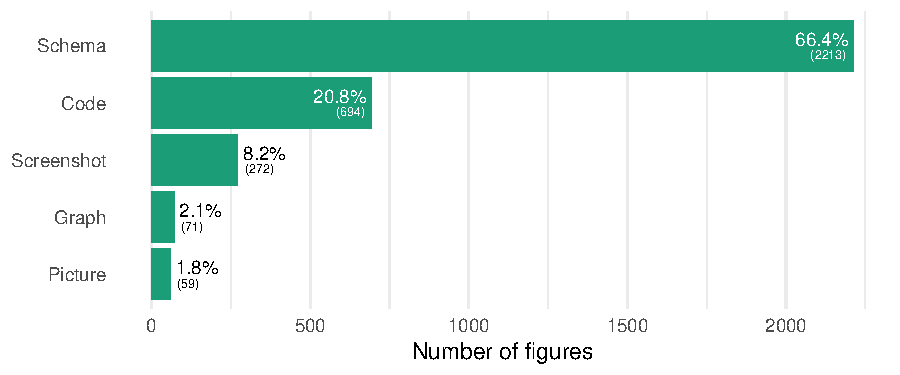
\includegraphics[keepaspectratio]{FiguresSE_files/figure-pdf/fig-nonq-1.pdf}}

}

\caption{\label{fig-nonq}Type of non quantitative figures}

\end{figure}%

\subsection{RQ3 Types}\label{rq3-types}

We report in Fig.~\ref{fig-quantitative} the overall proportion of the
different types of quantitative figures present in our taxonomy.

\phantomsection\label{cell-fig-quantitative}
\begin{figure}[tb]

\centering{

\pandocbounded{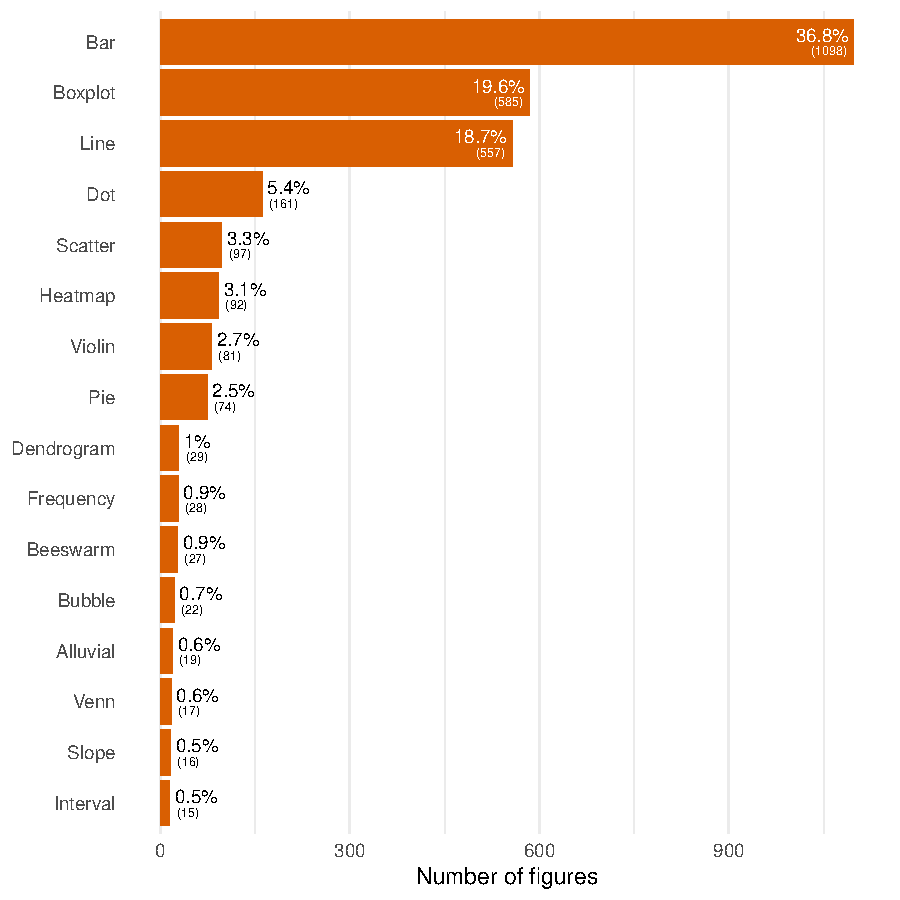
\includegraphics[keepaspectratio]{FiguresSE_files/figure-pdf/fig-quantitative-1.pdf}}

}

\caption{\label{fig-quantitative}Type of quantitative figures}

\end{figure}%

Overall one of every three quantitative figures contains a bar plot The
two other common used plot types are boxplots (19.6\%) and line plots
(18.7\%). Dot plots and scatter plots together make 8.8\%, heatmaps
account for 3.1\% of quantitative figures, the remaining types overall
account for 13\% of quantitative diagram, any of them accounting for
less than 3\% individually.

In the taxonomy we used for quantitative diagram types -- reported in
Section~\ref{sec-variables} --, we have different types of bar plots.
Fig.~\ref{fig-bars} reports the number and the proportion of the
different type of bar charts. Apart the simple bar charts that are used
in half of the cases, one in four bar diagram use grouped or clustered
bars, and 17\% use stacked bars. A small minority of bar diagram are
diverging diagrams.

\phantomsection\label{cell-fig-bars}
\begin{figure}[tb]

\centering{

\pandocbounded{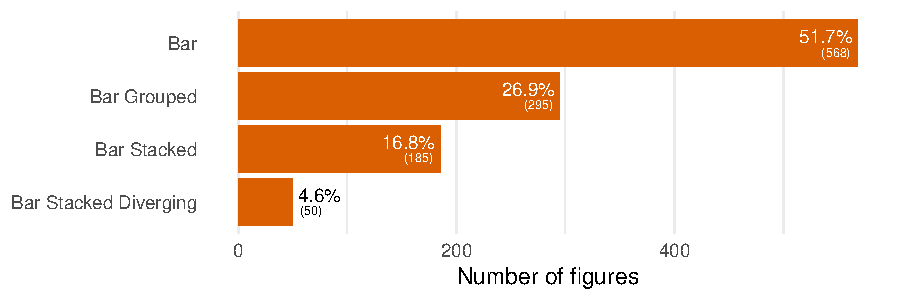
\includegraphics[keepaspectratio]{FiguresSE_files/figure-pdf/fig-bars-1.pdf}}

}

\caption{\label{fig-bars}Specific sub-types of bar graphs}

\end{figure}%

\subsection{RQ4: Errors}\label{rq4-errors}

On the basis of the error taxonomy described in section
Section~\ref{sec-error-taxonomy} we detected the errors committed in the
quantitative figures. The violin plots in
Fig.~\ref{fig-error-venue-distr} describe the distribution of errors per
quantitative figure detected in the articles appearing in the four
considered venues.

\phantomsection\label{cell-fig-error-venue-distr}
\begin{figure}[tb]

\centering{

\pandocbounded{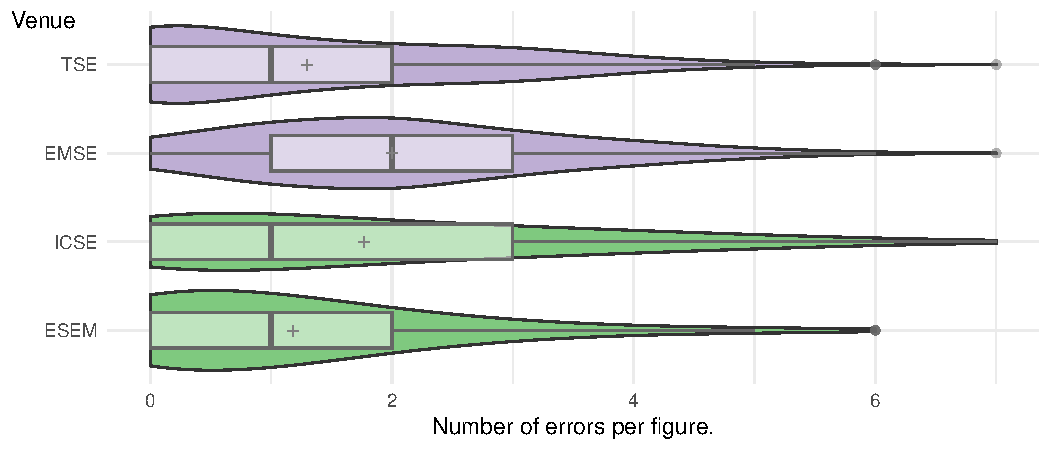
\includegraphics[keepaspectratio]{FiguresSE_files/figure-pdf/fig-error-venue-distr-1.pdf}}

}

\caption{\label{fig-error-venue-distr}Number of errors per figure by
venue}

\end{figure}%

We observe the average number of errors per figure is 1.6 (median 1).
Overall half of the figures exhibit at least one error, with half the
EMSE articles showing at least 2 errors. Concerning the proportion of
figures where no error was detected, they are 37.4\% for ESEM,30.6\% for
ICSE,12.2\% for EMSE,40.1\% for TSE.

A more detailed picture can be gained by looking at the frequency of
error free figures by severity level and venue reported in
Table~\ref{tbl-severity-error-free}.

\begin{table}

\caption{\label{tbl-severity-error-free}Proportion of error free figures
per severity and venue}

\centering{

\begin{tabular}[t]{llll}
\toprule
Venue & Critical & Major & Minor\\
\midrule
ESEM & 79.3\% & 64.6\% & 62.0\%\\
ICSE & 77.9\% & 49.2\% & 54.4\%\\
EMSE & 74.3\% & 40.3\% & 41.1\%\\
TSE & 77.5\% & 65.2\% & 60.1\%\\
\bottomrule
\end{tabular}

}

\end{table}%

Overall we observe that one every four pictures contains at least a
critical error, with similar condition across the four venues.
Concerning the major errors, the journal TSE and the conference ESEM
contain at least one error in one out of three figures, while the
proportion of figures with at least one major error is 50\% for ICSE and
60\% for EMSE. As far as minor errors are concerned, we observe a
similar amount of defective figures for all venues except EMSE where
60\% of figures contain at least one error.

Focusing down more, from the severity levels to the specific types of
errors, Fig.~\ref{fig-error-type} reports the occurrence numbers and
proportions of all the error types defined in the error taxonomy we
defined in Section~\ref{sec-error-taxonomy}. The errors types are
reported divided by severity levels.

\phantomsection\label{cell-fig-error-type}
\begin{figure}[tb]

\centering{

\pandocbounded{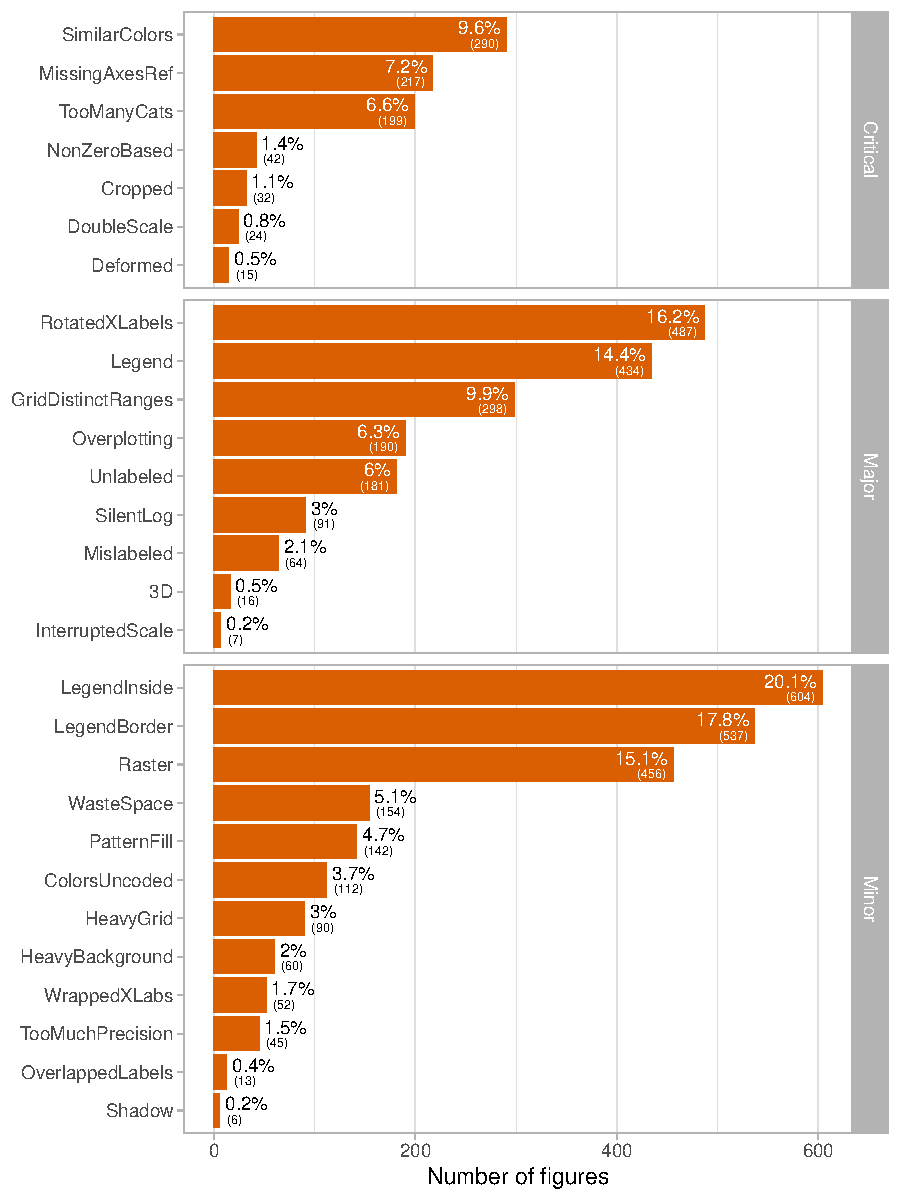
\includegraphics[keepaspectratio]{FiguresSE_files/figure-pdf/fig-error-type-1.pdf}}

}

\caption{\label{fig-error-type}Overall frequency of error committed in
quantitative figures}

\end{figure}%

As far as the major errors are concerned, we observe that the most
common error -- affecting 9.6\% of figures -- is the adoption of a
colour palette that does not enable an easy distinction of categories.
The next error consists in missing references on the axes (7.2\%), and
eventually the attempt to encode too many distinct categories in a
single plot (6.6\%).

The most common major error is the use of rotated labels on the x axis
(16.2\%), next is the use of a legend instead of direct labelling
(14.4\%). The next error affects figures containing multiple diagrams
and consists in using different scales on aligned diagrams (9.9\%).

The two most common minor errors regard the use of legends, often (20\%
of figures) the legend is placed inside the plot, which reduces the
clarity, also (17.8\%) the legend is surrounded by a border that affects
the ease of scanning back and forth between plot and legend itself.
Another common error is the use of raster images (15.1\%) that affects
the overall visual quality of the diagram.

\section{Discussion}\label{discussion}

Based on the findings reported in the previous section we can answer the
original research questions of the research and outline a few additional
considerations.

\subsection{Answers to Research
Questions}\label{answers-to-research-questions}

As far as the mode of use of figures (RQ1) is concerned, we observed a
relatively large adoption of figures with an average of 0.42 figures per
page. As a comparison the present paper contains 12 figures in 8 pages,
that is 1.5 figures per page, a clear outlier if we look at
Fig.~\ref{fig-density}. Two venues are aligned with the average (ESEM
and TSE) while the two other depart significantly: ICSE has higher
density while EMSE has lower density. Concerning this latter difference,
it can be explained by the larger number of pages of the articles
published by EMSE.

\begin{tcolorbox}[enhanced jigsaw, bottomrule=.15mm, breakable, colframe=quarto-callout-note-color-frame, toprule=.15mm, arc=.35mm, colback=white, rightrule=.15mm, leftrule=.75mm, opacityback=0, left=2mm]

\vspace{-3mm}\textbf{RQ1: how are figures used in SE articles?}\vspace{3mm}

On average, there are two figures every five pages with some difference
among venues, partly due to the length of articles.

\end{tcolorbox}

Concerning the category of figures -- quantitative vs.~non-quantitative
--, we found that 47\% of figures is quantitative but there are large
difference among the three considered venues. Articles appearing in ICSE
have just 1/3 of Q figures while ESEM papers have 2/3. A possible
explanation for such difference is that since ESEM is hosting mainly
empirical studies, the authors often need to show quantitative
information and Q figures are widely -- 44\% of papers contain only
quantitative figures -- used for this purpose. On the other hand, ICSE
hosts papers that have less empirical content and thus employ Q figures
less, moreover the wide spectrum of topics present at ICSE require to
provide context and details that are better explained with diagrams;
such use of overview diagrams could explain the higher number of figures
in ICSE papers, in fact the proportion of articles without quantitative
figures is simila in ICSE and ESEM.

\begin{tcolorbox}[enhanced jigsaw, bottomrule=.15mm, breakable, colframe=quarto-callout-note-color-frame, toprule=.15mm, arc=.35mm, colback=white, rightrule=.15mm, leftrule=.75mm, opacityback=0, left=2mm]

\vspace{-3mm}\textbf{RQ2: what are figures used for?}\vspace{3mm}

A bit less than half of the figures are used to convey quantitative
information, with wide variation from 1/3 to 2/3. Overall one in five
papers have no quantitative figure at all; while only 6\% of papers
contain only quantitative figures, with the notable exception of ESEM
conference where 44\% articles do.

\end{tcolorbox}

When looking at the type of quantitative diagrams used, we observe that
more than one in three is a bar plot (36.8\%). The second most used
diagram type are boxplots (19.6\%), in fact showing the distribution of
a set of values is a common necessity in empirical studies. Other means
to show distributions are violin plots (2.7\%) and beeswarm (0.9\%), in
addition to histograms that in our taxonomy are conflated with bar
plots. Line plots represent the third most common type of quantitative
diagram (18.7\%). They address the common requirement of showing trends
and relationships between pairs of variables. Scatter plots that have
similar use are much less common (3.3\%). Other types of diagram that
are known for perceptual issues, that is pies and bubbles, are rarely
used: 2.5\% and 0.7\% respectively.

\begin{tcolorbox}[enhanced jigsaw, bottomrule=.15mm, breakable, colframe=quarto-callout-note-color-frame, toprule=.15mm, arc=.35mm, colback=white, rightrule=.15mm, leftrule=.75mm, opacityback=0, left=2mm]

\vspace{-3mm}\textbf{RQ3: what type of quantitive diagrams are used?}\vspace{3mm}

The most common type is bar plot, used in one out of three figures,
followed by boxplots and line plots, each used in 20\% of figures.

\end{tcolorbox}

Talking about errors, we found 1.6 errors per figure on average (median
1). Anyway, across all venues, one in three figures showed no errors
according to our taxonomy, while considering only critical errors, three
out of four figures are fine. Focusing on major and minor errors, we
observed that half of the figures showed at least one.

The use of colours too similar to each other is the most common critical
error, this is often due to little care spent in selecting an
appropriate palette. The lack of values on the axes is another
relatively common error that has a heavy impact on the ability to
understand the diagram. Often in graphs that have been generated by
basic tools -- e.g.~spreadsheet programs --, the categories are
automatically encoded using many different variation of a single visual
attribute -- e.g.~shape or color -- that require a lot of cognitive
effort to be discerned. A little more design effort should be spent in
finding alternative representations that make understanding more
immediate. Another common result of using unaltered graphs produced by
e.g.~spreadsheets is having rotated or slanted labels on the x axis,
making reading the graph more difficult than required. Most of the time
a simple solution is to swap x and y axes; this should be the immediate
choice in presence of long labels. Another common mistake that is worth
mentioning is the use of a legend instead of direct labelling the series
of data in the plot area. This is probably due to the default in most
tools as well as the difficulty in implementing direct labelling in
those tools.

Most of the times errors could be solved with a small effort. We believe
they are introduce because authors do not pay enough attention to the
quality of the figures and, in the case of journals, neither the
reviewers do. Some basic and easy to follow guidelines are presented in
the Empirical Standards for Software Engineering Research
\citeproc{ref-EmpiricalStandards}{{[}3{]}}.

We note that very few figures show evident mistakes such as using
non-zero based bars, copping figures, adopting double scales or
deforming the graph area; still almost 5\% of figures are affected.

\begin{tcolorbox}[enhanced jigsaw, bottomrule=.15mm, breakable, colframe=quarto-callout-note-color-frame, toprule=.15mm, arc=.35mm, colback=white, rightrule=.15mm, leftrule=.75mm, opacityback=0, left=2mm]

\vspace{-3mm}\textbf{RQ4: what errors are found in quantitative figures?}\vspace{3mm}

The average figure in SE articles contains one or two errors, although
on average 1/3 of figures show no error. A common critical error is the
use of hard to discern palettes. The use of rotated labels on the x axis
is the most widespread major error. Common minor errors include a less
than ideal use of legends.

\end{tcolorbox}

\subsection{Limitations}\label{limitations}

The study presented in this paper is exploratory and therefore presents
several limitations; we highlight the main ones.

Only a few selected SE publication venues have been considered. Although
the venues have a very good reputation, they do not represent the whole
publication spectrum in SE. Moreover the articles have been drawn from a
limited time span, they represent a sample. This might affect the
external validity of the study. The graph error taxonomy has been built
based on the literature in the area of data visualization, although it
has not been empirically validates. It could have omitted important
errors or, vice-versa, considered error that are not such in the view of
other researchers. In addition the severity level has been assigned to
each error on the basis of the author expert judgment. In the
classification of the type of quantitative diagrams we considered only
the main type, although there are several cases of diagram that mix
multiple types, e.g.~bars + lines, that were not considered.

\section{Conclusions}\label{conclusions}

In this work we collected articles from four leading SE publication
venues, two conferences and two journals, and analyzed how figures are
used. We found the average density is 0.42 figures per page and half of
them are used to convey quantitative information. The most common
quantitative graph types are bar plots, boxplots, and line plots. We
also classified the errors committed in the quantitative graphs and we
found that on average every figure has 1 or 2 errors.

Most errors are relatively easy to address and we advocate for a wider
diffusion of visual literacy in the SE research community.

As future work we would like to extend the survey to a wider time span
as well as other venues. In addition we should take into consideration
figures with multiple types. Eventually, a pragmatic guide to assess and
improve quantitative diagrams and help researchers avoid the most common
pitfalls, could be defined based on this work.

\section*{References}\label{references}
\addcontentsline{toc}{section}{References}

\phantomsection\label{refs}
\begin{CSLReferences}{0}{0}
\bibitem[\citeproctext]{ref-tufte1983}
\CSLLeftMargin{{[}1{]} }%
\CSLRightInline{E. R. Tufte, \emph{The visual display of quantitative
information}. Graphics Press, 1983. }

\bibitem[\citeproctext]{ref-munzner2014}
\CSLLeftMargin{{[}2{]} }%
\CSLRightInline{T. Munzner, \emph{Visualization analysis and design}.
CRC Press, 2014. }

\bibitem[\citeproctext]{ref-EmpiricalStandards}
\CSLLeftMargin{{[}3{]} }%
\CSLRightInline{P. Ralph \emph{et al.}, {``Empirical standards for
software engineering research.''} 2021 {[}Online{]}. Available:
\url{https://arxiv.org/abs/2010.03525}}

\bibitem[\citeproctext]{ref-pandey2015}
\CSLLeftMargin{{[}4{]} }%
\CSLRightInline{A. V. Pandey, K. Rall, M. L. Satterthwaite, O. Nov, and
E. Bertini, {``\href{https://doi.org/10.1145/2702123.2702608}{How
deceptive are deceptive visualizations? An empirical analysis of common
distortion techniques},''} in \emph{Proceedings of the 33rd annual ACM
conference on human factors in computing systems}, 2015, pp. 1469--1478.
}

\bibitem[\citeproctext]{ref-Few2012}
\CSLLeftMargin{{[}5{]} }%
\CSLRightInline{S. Few, \emph{Show me the numbers, second edition}.
Analytics Press, 2012. }

\bibitem[\citeproctext]{ref-ware2013}
\CSLLeftMargin{{[}6{]} }%
\CSLRightInline{C. Ware, \emph{Information visualization: Perception for
design}. Elsevier Science, 2013. }

\bibitem[\citeproctext]{ref-silva2011}
\CSLLeftMargin{{[}7{]} }%
\CSLRightInline{S. Silva, B. S. Santos, and J. Madeira,
{``\href{https://doi.org/10.1016/j.cag.2010.11.015}{Using color in
visualization: A survey},''} \emph{Computers \& Graphics}, vol. 35, no.
2, pp. 320--333, 2011. }

\bibitem[\citeproctext]{ref-macdonald1999}
\CSLLeftMargin{{[}8{]} }%
\CSLRightInline{L. W. MacDonald,
{``\href{https://doi.org/10.1109/38.773961}{Using color effectively in
computer graphics},''} \emph{IEEE Computer Graphics and Applications},
vol. 19, no. 4, pp. 20--35, 1999. }

\bibitem[\citeproctext]{ref-heer2009}
\CSLLeftMargin{{[}9{]} }%
\CSLRightInline{J. Heer, F. B. Viégas, and M. Wattenberg,
{``\href{https://doi.org/10.1145/1435417.1435439}{Voyagers and voyeurs:
Supporting asynchronous collaborative visualization},''}
\emph{Communications of the ACM}, vol. 52, no. 1, pp. 87--97, 2009. }

\bibitem[\citeproctext]{ref-ratwani2008}
\CSLLeftMargin{{[}10{]} }%
\CSLRightInline{R. M. Ratwani, J. G. Trafton, and D. A. Boehm-Davis,
{``\href{https://doi.org/10.1037/1076-898X.14.1.36}{Thinking
graphically: Connecting vision and cognition during graph
comprehension},''} \emph{Journal of Experimental Psychology: Applied},
vol. 14, no. 1, p. 36, 2008. }

\bibitem[\citeproctext]{ref-cleveland1994}
\CSLLeftMargin{{[}11{]} }%
\CSLRightInline{W. S. Cleveland, \emph{The elements of graphing data}.
AT\&T Bell Laboratories, 1994. }

\bibitem[\citeproctext]{ref-GQM1999}
\CSLLeftMargin{{[}12{]} }%
\CSLRightInline{R. van Solingen and E. W. Berghout, \emph{The
goal/question/metric method: A practical guide for quality improvement
of software development}. McGraw-Hill, 1999. }

\end{CSLReferences}


% Can use something like this to put references on a page
% by themselves when using endfloat and the captionsoff option.
\ifCLASSOPTIONcaptionsoff
  \newpage
\fi

% trigger a \newpage just before the given reference
% number - used to balance the columns on the last page
% adjust value as needed - may need to be readjusted if
% the document is modified later
%\IEEEtriggeratref{8}
% The "triggered" command can be changed if desired:
%\IEEEtriggercmd{\enlargethispage{-5in}}

% Uncomment when use biblatex with style=ieee
%\renewcommand{\bibfont}{\footnotesize} % for IEEE bibfont size

\pagebreak[3]
% that's all folks
\end{document}

